\documentclass[10pt]{beamer}

\newcommand{\lectnum}{L12}
\newcommand{\lecttitle}{The EM algorithm}

\usepackage{amsmath, amssymb, graphicx}
\usepackage[]{algorithm2e}
\usepackage{pdfpages}
\usepackage[british]{babel}

\hypersetup{colorlinks,linkcolor=,urlcolor=blue}
\newenvironment{titledslide}[1]{\begin{frame}\frametitle{#1}}{\end{frame}}

\mode<presentation>{\setbeamercovered{transparent}}

\setbeamertemplate{sidebar right}{}
\setbeamertemplate{footline}{%
\hfill\usebeamertemplate***{navigation symbols}
\hspace{0.4cm}\lectnum: \insertframenumber{}/\inserttotalframenumber \hspace*{0.4cm}}

\author{James Cussens}

\title{COMS30035, Machine learning:\\ \vspace{5pt} \lecttitle}

\institute{School of Computer Science\\University of Bristol}

\begin{document}
%%%%%%%%%%%%%%%%%%%%%%%%%%%%%%%%%%%%%%%%%%%%%%%%%%%%%%%%%%%%%%%%%%%%%%

\begin{frame}
  \titlepage
\end{frame}

%%%%%%%%%%%%%%%%%%%%%%%%%%%%%%%%%%%%%%%%%%%%%%%%%%%%%%%%%%%%%%%%%%%%%%

\usetikzlibrary{bayesnet}

\newcommand{\xvec}{\ensuremath{\mathbf{x}}}
\newcommand{\Xvec}{\ensuremath{\mathbf{X}}}
\newcommand{\Zvec}{\ensuremath{\mathbf{Z}}}
\newcommand{\thetavec}{\ensuremath{{\bm \theta}}}
\newcommand{\xvecn}{\ensuremath{\mathbf{x}_{n}}}
\newcommand{\zvec}{\ensuremath{\mathbf{z}}}
\newcommand{\bmu}{\ensuremath{{\bm \mu}}}
\newcommand{\bcov}{\ensuremath{{\bm \Sigma}}}
\newcommand{\gauss}{\ensuremath{{\cal N}}}


%%%%%%%%%%%%%%%%%%%%%%%%%%%%%%%%%%%%%%%%%%%%%%%%%%%%%%%%%%%%%%%%%%%%%%
\begin{titledslide}{MLE for a Gaussian mixture}

 
  \begin{equation*}
    \label{eq:loglik}
    \ln p(\Xvec|{\bm \pi}, \bmu, {\bm \Sigma}) = \sum_{n=1}^{N} \ln
     \left\{ \sum_{k=1}^{K} \pi_{k} \gauss(\xvec_{n}|\bmu_{k},{\bm \Sigma}_{k}) \right\}  
  \end{equation*}

  \begin{itemize}
  \item No closed form for the MLE
  \item (At least $K!$ solutions)	
  \item So have to resort to an iterative algorithm.
  \item ``It should be emphasized that there will generally be
    multiple local maxima of the log likelihood function'' \cite[p. 438]{bishop06:_patter_recog_machin_learn}.
  \item The iterative algorithm we use is called the
    \emph{Expectation-Maximization (EM) algorithm}.
  
  \end{itemize}
  
\end{titledslide}

\begin{titledslide}{Settings derivatives to zero}

 %\begin{equation*}
   % \ln p(\Xvec|{\bm \pi}, \bmu, {\bm \Sigma}) = \sum_{n=1}^{N} \ln
     %\left\{ \sum_{k=1}^{K} \pi_{k} \gauss(\xvec_{n}|\bmu_{k},{\bm \Sigma}_{k}) \right\}  
  %\end{equation*}

\begin{eqnarray*}
\bmu_{k} & = & \frac{1}{N_{k}} \sum_{n=1}^{N} \gamma(z_{nk}) \xvec_{n} \\
{\bm \Sigma}_{k} & = & \frac{1}{N_{k}} \sum_{n=1}^{N} \gamma(z_{nk}) (\xvec_{n} - \bmu_{k})(\xvec_{n} - \bmu_{k})^{T} \\
\pi_{k} & = & \frac{N_{k}}{N}
\end{eqnarray*}

where $\gamma(z_{nk}) = p(z_{k}=1|\xvec_{n})$ and $N_{k} = \sum_{n=1}^{N} \gamma(z_{nk}) $.

\vspace{0.8cm}

\begin{itemize}
\item See \cite[\S 9.22]{bishop06:_patter_recog_machin_learn} for the derivation.
\end{itemize}

\end{titledslide} 
\begin{titledslide}{EM for Gaussian mixtures}

\begin{itemize}
\item To initialise the EM algorithm we choose starting values for $\bmu$, ${\bm \Sigma}$ and $\pi$.
\end{itemize}


\textbf{E step} Compute the values for the responsibilities $\gamma(z_{nk})$ given the current parameter values:

\[
\gamma(z_{nk}) = \frac{
\pi_{k} \gauss(\xvec_{n}|\bmu_{k},{\bm \Sigma}_{k})
}
{\sum_{j=1}^{K} \pi_{j} \gauss(\xvec_{n}|\bmu_{j},{\bm \Sigma}_{j})}
\]

\textbf{M step} Re-estimate the parameters using the current responsibilities:
\begin{eqnarray*}
\bmu_{k}^{\mbox{new}} & = & \frac{1}{N_{k}} \sum_{n=1}^{N} \gamma(z_{nk}) \xvec_{n} \\
{\bm \Sigma}_{k}^{\mbox{new}} & = & \frac{1}{N_{k}} \sum_{n=1}^{N} \gamma(z_{nk}) (\xvec_{n} - \bmu_{k}^{\mbox{new}})(\xvec_{n} - \bmu_{k}^{\mbox{new}})^{T} \\
\pi_{k}^{\mbox{new}} & = & \frac{N_{k}}{N}
\end{eqnarray*}


\end{titledslide}
%%%%%%%%%%%%%%%%%%%%%%%%%%%%%%%%%%%%%%%%%%%%%%%%%%%%%%%%%%%%%%%%%%%%%%
\begin{titledslide}{This E-step is just Bayes theorem}

  \[
    p(z_{k}=1|\xvec_{n}) =
    \frac{p(z_{k}=1)p(\xvec_{n}|z_{k}=1)}{p(\xvec_{n})}
    = \frac{p(z_{k}=1)p(\xvec_{n}|z_{k}=1)}{\sum_{j=1}^{K}p(z_{j}=1)p(\xvec_{n}|z_{j}=1)}
  \]
  
The same equation in different notation is:
  
  \[
    \gamma(z_{nk}) = \frac{
      \pi_{k} \gauss(\xvec_{n}|\bmu_{k},{\bm \Sigma}_{k})
    }
    {\sum_{j=1}^{K} \pi_{j} \gauss(\xvec_{n}|\bmu_{j},{\bm \Sigma}_{j})}
  \]

  
\end{titledslide}
%%%%%%%%%%%%%%%%%%%%%%%%%%%%%%%%%%%%%%%%%%%%%%%%%%%%%%%%%%%%%%%%%%%%%%
\begin{titledslide}{EM in pictures}

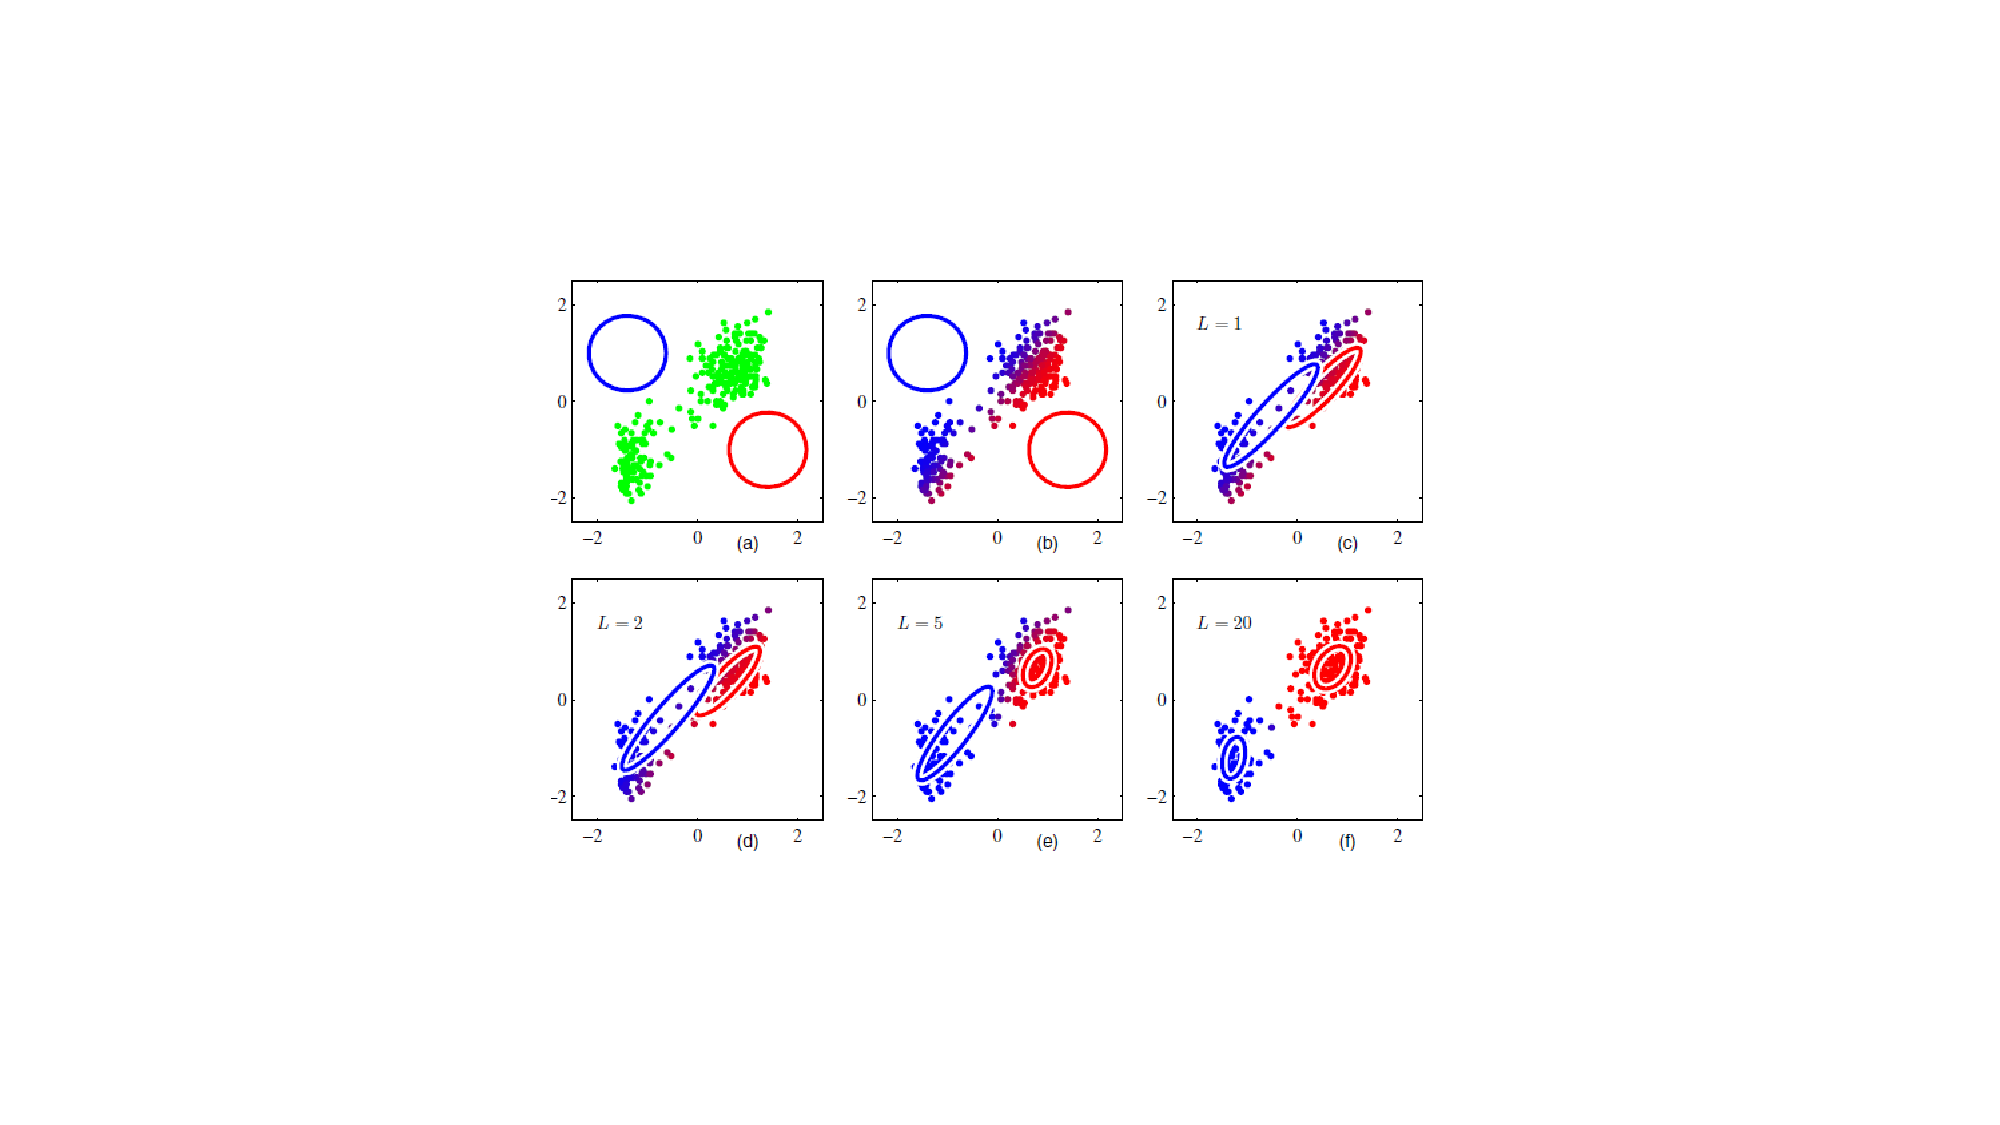
\includegraphics[trim=2.8in 2in 2in 1.8in,width=1.2\textwidth,clip]{../figures/emplots.pdf}


\end{titledslide} 
%%%%%%%%%%%%%%%%%%%%%%%%%%%%%%%%%%%%%%%%%%%%%%%%%%%%%%%%%%%%%%%%%%%%%%
\begin{titledslide}{Why does EM work?}

  \begin{itemize}
  \item We have yet to show that each iteration of the EM algorithm
    increases the log-likelihood $\ln p(\Xvec|{\bm \pi}, \bmu, {\bm
      \Sigma})$.
  \item We will do this for the general case: 
  \end{itemize}


\begin{equation*}
\ln p(\Xvec | \thetavec) = \ln \left\{ \sum_{\zvec} p(\Xvec,\Zvec| \thetavec) \right\}
\end{equation*}
\begin{itemize}
\item $Z$ are hidden variables (i.e.\ not observed) also called
  \emph{latent variables}.
\item $\{X,Z\}$ is the \emph{complete data}. Assume that if we had the complete data then MLE would be easy.
\item $\{X\}$ is the \emph{incomplete data}.
\end{itemize}
\end{titledslide}
%%%%%%%%%%%%%%%%%%%%%%%%%%%%%%%%%%%%%%%%%%%%%%%%%%%%%%%%%%%%%%%%%%%%%%
\begin{titledslide}{Decomposing the log-likelihood}

  \begin{itemize}
  \item Let $q(\Zvec)$ be any distribution over the hidden variables.
  \item We have the following key decomposition of the log-likelihood:
  \end{itemize}

  \[
    \ln p(\Xvec | \thetavec)  = {\cal L}(q, \thetavec) + \mathrm{KL}(q
      || p)
  \]
  where
  \begin{eqnarray*}
    {\cal L}(q, \thetavec) & = & \sum_{\Zvec} q(\Zvec) \ln \left\{
      \frac{p(\Xvec,\Zvec| \thetavec)}{q(\Zvec)} \right\} \\
    \mathrm{KL}(q || p) & = & -\sum_{\Zvec} q(\Zvec) \ln \left\{
      \frac{p(\Zvec|\Xvec, \thetavec)}{q(\Zvec)} \right\}
  \end{eqnarray*}

  \begin{itemize}
  \item An exercise for you: prove that this decomposition is correct
    (Exercise 9.24 in Bishop). Use the tip Bishop gives on p.451.
  \end{itemize}

  
\end{titledslide}
%%%%%%%%%%%%%%%%%%%%%%%%%%%%%%%%%%%%%%%%%%%%%%%%%%%%%%%%%%%%%%%%%%%%%%
\begin{titledslide}{Kullback-Leibler divergence}

  \[
    \mathrm{KL}(q || p)  =  -\sum_{\Zvec} q(\Zvec) \ln \left\{
      \frac{p(\Zvec|\Xvec, \thetavec)}{q(\Zvec)} \right\}
  \]
  
  \begin{itemize}
  \item   $\mathrm{KL}(p_{1} || p_{2})$ denotes the
    \emph{Kullback-Leibler divergence} between probability
    distributions $p_1$ and $p_2$.
  \item KL-divergence is important in, e.g., information theory.
  \item It's a bit like a `distance' between two distributions.
  \item But it is not a true distance since, for example, it is not
    symmetric.
  \item $\mathrm{KL}(p_{1} || p_{2}) \geq 0$ and $\mathrm{KL}(p_{1} ||
    p_{2}) = 0$ if and only if $p_{1}=p_{2}$. 
  \end{itemize}
  
\end{titledslide}
%%%%%%%%%%%%%%%%%%%%%%%%%%%%%%%%%%%%%%%%%%%%%%%%%%%%%%%%%%%%%%%%%%%%%%
\begin{titledslide}{EM: key ideas}

  \[
    \ln p(\Xvec | \thetavec)  = {\cal L}(q, \thetavec) + \mathrm{KL}(q
      || p)
  \]

  \begin{itemize}
  \item $\mathrm{KL}(q
      || p) \geq 0$ for any choice of $q$, so ${\cal L}(q, \thetavec)
      \leq \ln p(\Xvec | \thetavec)$.
    \item In the E-step we increase ${\cal L}(q, \thetavec)$ by
      updating $q$ (and leaving $\thetavec$ fixed).
    \item In the M-step we increase ${\cal L}(q, \thetavec)$ by
      updating $\thetavec$ (and leaving $q$ fixed).
    \item After the E-step we have
      ${\cal L}(q, \thetavec) = \ln p(\Xvec | \thetavec)$, so that in
      the following M-step increasing ${\cal L}(q, \thetavec)$ will
      also increase $\ln p(\Xvec | \thetavec)$.
  \end{itemize}
  
\end{titledslide}
%%%%%%%%%%%%%%%%%%%%%%%%%%%%%%%%%%%%%%%%%%%%%%%%%%%%%%%%%%%%%%%%%%%%%%
\begin{titledslide}{The E-step}

  \[
    \ln p(\Xvec | \thetavec^{\mbox{old}})  = {\cal L}(q, \thetavec^{\mbox{old}}) + \mathrm{KL}(q
      || p)
  \]
  
  \begin{itemize}
  \item In the E-step we update $q$ but leave $\thetavec^{\mbox{old}}$ fixed. 
  \item $\mathrm{KL}(q
      || p) = 0$ when $q=p$, so to maximise ${\cal L}(q,
      \thetavec^{\mbox{old}})$ we set $q(\Zvec) = p(\Zvec|\Xvec,
      \thetavec^{\mbox{old}})$.
    \item This increases ${\cal L}(q, \thetavec^{\mbox{old}})$ but not
      $\ln p(\Xvec | \thetavec^{\mbox{old}})$.
    \item \cite[Fig~9.12]{bishop06:_patter_recog_machin_learn}
      illustrates the E-step.
  \end{itemize}
  
\end{titledslide}
%%%%%%%%%%%%%%%%%%%%%%%%%%%%%%%%%%%%%%%%%%%%%%%%%%%%%%%%%%%%%%%%%%%%%%
\begin{titledslide}{The M-step}

  \[
    \ln p(\Xvec | \thetavec^{\mbox{new}})  = {\cal L}(q, \thetavec^{\mbox{new}}) + \mathrm{KL}(q
      || p)
  \]
  \[
    {\cal L}(q, \thetavec) =  \sum_{\Zvec} q(\Zvec) \ln \left\{
      \frac{p(\Xvec,\Zvec| \thetavec)}{q(\Zvec)} \right\} = \sum_{\Zvec} q(\Zvec) \ln \
      p(\Xvec,\Zvec| \thetavec) -  \sum_{\Zvec} q(\Zvec) \ln q(\Zvec)
  \]

  
  \begin{itemize}
  \item In the M-step we find parameters $\thetavec^{\mbox{new}}$
    which maximise  ${\cal L}(q, \thetavec)$, while leaving $q$ fixed.
  \item This will necessarily increase $\ln p(\Xvec | \thetavec)$
    since  $\mathrm{KL}(q
    || p) \geq 0 $.
  \item In fact we get a `bonus' since changing $p$ from $p(\Zvec|\Xvec,
    \thetavec^{\mbox{old}})$ to $p(\Zvec|\Xvec,
    \thetavec^{\mbox{new}})$ will (typically) lead  $\mathrm{KL}(q
    || p)$ to increase from 0 to some positive value.
  \item \cite[Fig~9.13]{bishop06:_patter_recog_machin_learn}
    illustrates the M-step.
  \end{itemize}
\end{titledslide}
%%%%%%%%%%%%%%%%%%%%%%%%%%%%%%%%%%%%%%%%%%%%%%%%%%%%%%%%%%%%%%%%%%%%%%
\begin{titledslide}{Visualising EM}

  \begin{itemize}
  \item David Barber (from UCL) provides a nice visualisation for EM (where the
    latent variable is binary).
  \item It's Fig~11.2 on p.259 of his \href{http://web4.cs.ucl.ac.uk/staff/D.Barber/textbook/200620.pdf}{book} \cite{barber12:_bayes_reason_machin_learn}.
  \end{itemize}
  
\end{titledslide}
%%%%%%%%%%%%%%%%%%%%%%%%%%%%%%%%%%%%%%%%%%%%%%%%%%%%%%%%%%%%%%%%%%%%%% 
\begin{titledslide}{Back to Gaussian mixtures}

  \begin{itemize}
  \item In the standard case of independent and identically
    distributed (i.i.d.) dataset $\Xvec$, we get:
  \end{itemize}
  \[
    p(\Zvec|\Xvec,
    \thetavec) = \prod_{n=1}^{N} p(\mathbf{z}_{n}|\mathbf{x}_n,\thetavec)
  \]
  \begin{itemize}
  \item In the case of Gaussian mixtures the responsibilities
    $\gamma(z_{nk})$ define the
    $p(\mathbf{z}_{n}|\mathbf{x}_n,\thetavec)$.
  \item So computing the responsibilities is the E-step.
  \item And the M-step we saw on slide 4 does indeed maximise
    ${\cal L}(q, \thetavec)$ given the current responsibilities.
  \item Proving this is Exercises 9.8 and 9.9 in Bishop.
  \end{itemize}
  
\end{titledslide}
%%%%%%%%%%%%%%%%%%%%%%%%%%%%%%%%%%%%%%%%%%%%%%%%%%%%%%%%%%%%%%%%%%%%%% 
\begin{titledslide}{Reading}

  \begin{itemize}
  \item Bishop \S9.2.2
  \item Bishop \S9.4
  \item Murphy \S8.7.2-\S8.7.3
  \end{itemize}
  
  
\end{titledslide}
%%%%%%%%%%%%%%%%%%%%%%%%%%%%%%%%%%%%%%%%%%%%%%%%%%%%%%%%%%%%%%%%%%%%%%
\begin{titledslide}{Problems and quizzes}

  \begin{itemize}
  \item Bishop Exercise 9.24 (Use the tip Bishop gives on p. 451)
  \item Quizzes:
    \begin{itemize}
    \item Week~5: The EM algorithm
    \end{itemize}
  \end{itemize}
  
\end{titledslide}
%%%%%%%%%%%%%%%%%%%%%%%%%%%%%%%%%%%%%%%%%%%%%%%%%%%%%%%%%%%%%%%%%%%%%%
\bibliographystyle{alpha}
\bibliography{../ml}


\end{document}
